
\sektion{
\includegraphics[height=0.6cm]{kotlin_logo_transparent}otlin in the wild}


%%%%%%%%%%%%%%%%%%%%%%%%%%%%%%%%%%%%%%%%%%%%%%%%
\begin{frame}[fragile] \frametitle{\texttt{build.gradle}}
\begin{lstlisting}
apply plugin: "kotlin"|\pause|
buildscript {
  ext.kotlin_version = '1.0.6'
  dependencies {
    classpath "org.jetbrains.kotlin:
      kotlin-gradle-plugin:$kotlin_version"
  }
}|\pause|
dependencies {
  compile "org.jetbrains.kotlin:
    kotlin-stdlib:$kotlin_version"
  compile "org.jetbrains.kotlin:
    kotlin-reflect:$kotlin_version"
}
\end{lstlisting}
\end{frame}

%%%%%%%%%%%%%%%%%%%%%%%%%%%%%%%%%%%%%%%%%%%%%%%%
\fullimageCapt{travis}{\href{https://travis-ci.org/christophpickl/gadsu}{travis-ci.org}}{10cm}

\begin{frame}[fragile] \frametitle{\texttt{.travis.yml}}
\begin{lstlisting}
language: kotlin|\pause|
sudo: false|\pause|
jdk:
  - oraclejdk8|\pause|
before_install:
  - "chmod +x gradlew"|\pause|
  - "export DISPLAY=:99.0"
  - "sh -e /etc/init.d/xvfb start"|\pause|
script:
  - "./gradlew test ..."|\pause|
notifications:
  email:
    - "MLtravis@gadsu.com"
\end{lstlisting}
\end{frame}

%%%%%%%%%%%%%%%%%%%%%%%%%%%%%%%%%%%%%%%%%%%%%%%%
\fullimageCapt{codecov}{\href{https://codecov.io/gh/christophpickl/gadsu/}{codecov.io}}{10cm}

\begin{frame}[fragile] \frametitle{Codecov} 
Gradle Configuration:

\begin{lstlisting}
plugins {
  id 'jacoco'
  id 'com.github.kt3k.coveralls'
}|\pause|
jacocoTestReport {
  reports {
    xml.enabled = true
}}
\end{lstlisting}
\pause

Travis Configuration:

\begin{lstlisting}
script:
  - "./gradlew ... jacocoTestReport ..."|\pause|
after_success:
  - bash <(curl -s https://codecov.io/bash)
\end{lstlisting}


\end{frame}


%%%%%%%%%%%%%%%%%%%%%%%%%%%%%%%%%%%%%%%%%%%%%%%%
\fullimageCapt{versioneye}{\href{https://www.versioneye.com/user/projects/572880644a0faa000b782062}{versioneye.com}}{10cm}

\begin{frame}[fragile] \frametitle{VersionEye} 
Gradle Configuration:
\begin{lstlisting}
plugins {
  id "org.standardout.versioneye"
    version "1.4.0"
}
\end{lstlisting}
\pause

Gradle Properties:
\begin{lstlisting}
versioneye.projectid=572880644a0f...00b78206
\end{lstlisting}
\pause


Travis Configuration:

\begin{lstlisting}
script:
  - "./gradlew ... versioneye-update ..."
\end{lstlisting}
 
\end{frame}


\begin{frame} \frametitle{VersionEye GitHub Integration} 

\centering{Display coverage data via the \href{https://github.com/codecov/browser-extension}{Codecov Browser Extension}:}

\begin{figure}[h]
\centering
  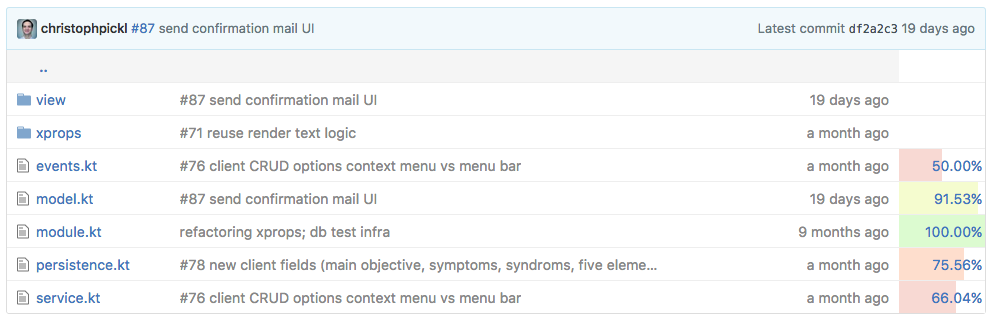
\includegraphics[width=10cm]{versioneye_github1}
\end{figure}
\begin{figure}[h]
\centering
  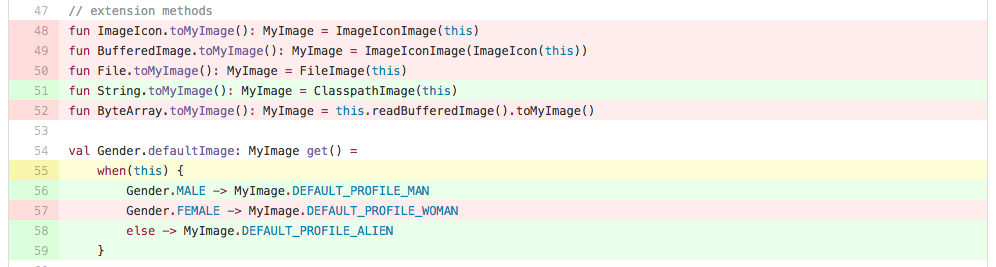
\includegraphics[width=10cm]{versioneye_github2}
\end{figure}
\end{frame}
